%----------------------------------------------------------------------------------------
%	PACKAGES AND OTHER DOCUMENT CONFIGURATIONS
%----------------------------------------------------------------------------------------

\documentclass[11pt, oneside]{Thesis} % The default font size and one-sided printing (no margin offsets)

\graphicspath{{Pictures/}} % Specifies the directory where pictures are stored

\usepackage{textcomp}
\usepackage[utf8]{inputenc}
\usepackage[square, numbers, comma, sort&compress]{natbib} % Use the natbib reference package - read up on this to edit the reference style; if you want text (e.g. Smith et al., 2012) for the in-text references (instead of numbers), remove 'numbers'
\usepackage[T1]{fontenc}
\usepackage{lmodern}
\usepackage{wrapfig}
\hypersetup{urlcolor=blue, colorlinks=true} % Colors hyperlinks in blue - change to black if annoying
\title{\ttitle} % Defines the thesis title - don't touch this

\begin{document}

\frontmatter % Use roman page numbering style (i, ii, iii, iv...) for the pre-content pages

\setstretch{1.3} % Line spacing of 1.3

% Define the page headers using the FancyHdr package and set up for one-sided printing
\fancyhead{} % Clears all page headers and footers
\rhead{\thepage} % Sets the right side header to show the page number
\lhead{} % Clears the left side page header

\pagestyle{fancy} % Finally, use the "fancy" page style to implement the FancyHdr headers

\newcommand{\HRule}{\rule{\linewidth}{0.5mm}} % New command to make the lines in the title page

% PDF meta-data
\hypersetup{pdftitle={\ttitle}}
\hypersetup{pdfsubject=\subjectname}
\hypersetup{pdfauthor=\authornames}
\hypersetup{pdfkeywords=\keywordnames}

%----------------------------------------------------------------------------------------
%	TITLE PAGE
%----------------------------------------------------------------------------------------

\begin{titlepage}
\begin{center}

\textsc{\LARGE \univname}\\[1.5cm] % University name
\textsc{\Large Rapport de stage}\\[0.5cm] % Thesis type

\HRule \\[0.4cm] % Horizontal line
{\huge \bfseries \ttitle}\\[0.4cm] % Thesis title
\HRule \\[1.5cm] % Horizontal line

\begin{minipage}{0.4\textwidth}
\begin{flushleft} \large
\emph{Auteur:}\\
\authornames % Author name - remove the \href bracket to remove the link
\end{flushleft}
\end{minipage}
\begin{minipage}{0.4\textwidth}
\begin{flushright} \large
\emph{Tuteur:} \\
\supname % Supervisor name - remove the \href bracket to remove the link
\end{flushright}
\end{minipage}\\[3cm]

\large \textit{Un rapport présentant le déroulement du stage au sein de FIGARO Classifieds \\ pour le diplôme d'ingénieur de l'EISTI}\\[0.3cm] % University requirement text

{\large \today}\\[4cm] % Date
%\includegraphics{Logo} % University/department logo - uncomment to place it

\vfill
\end{center}

\end{titlepage}

\clearpage % Start a new page

%----------------------------------------------------------------------------------------
%	ACKNOWLEDGEMENTS
%----------------------------------------------------------------------------------------

\setstretch{1.3} % Reset the line-spacing to 1.3 for body text (if it has changed)

\acknowledgements{\addtocontents{toc}{\vspace{1em}} % Add a gap in the Contents, for aesthetics

Merci à tous TODO \ldots
}
\clearpage % Start a new page

%----------------------------------------------------------------------------------------
%	LIST OF CONTENTS/FIGURES/TABLES PAGES
%----------------------------------------------------------------------------------------

\pagestyle{fancy} % The page style headers have been "empty" all this time, now use the "fancy" headers as defined before to bring them back

\lhead{\emph{Index}} % Set the left side page header to "Contents"
\tableofcontents % Write out the Table of Contents

\lhead{\emph{Liste des schémas}} % Set the left side page header to "List of Figures"
\listoffigures % Write out the List of Figures


%----------------------------------------------------------------------------------------
%	THESIS CONTENT - CHAPTERS
%----------------------------------------------------------------------------------------

\mainmatter % Begin numeric (1,2,3...) page numbering

\pagestyle{fancy} % Return the page headers back to the "fancy" style

% Include the chapters of the thesis as separate files from the Chapters folder
% Uncomment the lines as you write the chapters

% Chapter 1

\chapter{Recherche du stage} % Main chapter title

\label{presentation} % For referencing the chapter elsewhere, use \ref{presentation}

\lhead{Première partie. \emph{Présentation de l'entreprise}} % This is for the header on each page - perhaps a shortened title

%-------------------------------------------------------------------------------

\section{Introduction}

Le stage est une période très attendue de notre cursus au sein de l’EISTI car il nous permet de découvrir le monde du travail, notre futur métier et bien sûr d’appliquer les compétences que nous avons acquises tout au long de notre scolarité.
De plus, le stage de dernière année se déroule sur une période de plus de 20 semaines.
Cette durée permet d'exploiter les avantages d’un stage et nous permet d’avoir un recul important à l’issue de celui-ci.

%-------------------------------------------------------------------------------

\section{Ma démarche}
Le marché des offres de stage est bien plus caché que celui des offres d'emploi.
En effet, beaucoup d'offres ne sont pas publiées, ce qui rend la recherche bien compliquée.
Je vais expliquer dans la partie qui suit la façon dont j'ai procédé pour trouver mon stage de fin d'étude.

\subsection{Mes motivations}
J'ai effectué l'an dernier un stage dans une très grosse entreprise, comprenant des équipes importantes et utilisant des méthodes de management anciennes.
J'ai beaucoup travaillé seul en parfaite autonomie mais sans réels contacts avec les autres équipes.
Je souhaitais ainsi cette année effectuer mon stage dans une structure plus petite, de la taille d'une startup ou d'une PME.
Toujours en opposition avec ce stage précédent, je souhaitais travailler dans une équipe, sur des technologies nouvelles et en suivant des méthodes de management agiles.
Enfin, Scala est un langage qui m'a particulièrement intéressé cette année et l'utiliser pour les projets que nous avons effectués au cours de cette dernière année m'a motivé à chercher un stage dans lequel je pourrais m'y améliorer.

\subsection{Les entreprises contactées}
Le réseau de l'EISTI m'a proposé de nombreuses offres de stage différentes.
J'ai ainsi contacté des entreprises dont je recevais les offres par mail, qui étaient pour la plupart de grosses ESN.
Ces dernières sont connues pour employer assez facilement les eistiens; ainsi, bien que complètement éloignées des souhaits que j'ai énoncé, ces entreprises m'assuraient un stage.
J'ai aussi contacté quelques startup et PME, trouvées sur internet, en postulant à des offres de CDI ou en déposant des candidatures ouvertes.
J'ai contacté des entreprises implantées sur Pau, Toulouse et Bordeaux et quelques unes sur Paris.

\subsection{Les résultats de mes recherches}
J'ai reçu assez rapidement des réponses de la part des ESN contactées et même effectué quelques entretiens avec certaines, mais les sujets que l'on me présentait ne correspondaient pas à mes critères.
La plupart des projets se faisaient en J2E ou en C\#, langages qui ne m'intéressaient pas particulièrement, et les structures étaient grandes, ce qui nétait pas visé pour ce stage.
Les entreprises plus petites que j'ai contacté refusaient souvent mes demandes en tant que stagiaire puisqu'un CDI était recherché.
Une partie de ces entreprises m'ont recontactées pendant mon stage via le mail que je leur avais laissé ou bien via Linkedin.
FIGARO CLASSIFIEDS est l'une de ces PME que j'avais contacté pour un stage à la place d'un CDI.
L'entreprise m'a recontacté et nous avons organisé une rencontre via Skype très rapidement avec une responsable Ressources Humaines et monsieur Marc Morel, directeur informatique du pôle Carrière.
J'ai su rapidement, une semaine après l'envoi de mon premier mail, que j'étais retenu pour ce stage.

%-------------------------------------------------------------------------------

\section{Conclusion}

Grâce aux projets innovants réalisés tout au long de ma scolarité, au stage de deuxième année et à mon expérience universitaire en Ecosse, j'ai pu présenter aux entreprises que je rencontrais un CV intéressant pour un étudiant en fin de cursus, puisque mes expériences n'étaient pas uniquement théoriques et qu'elles étaient variées.
Ainsi j'ai eu la possibilité de choisir un stage qui m'intéressait parmi plusieurs offres.

% Chapter 2

\chapter{L'environnement du stage} % Main chapter title

\label{environnement} % For referencing the chapter elsewhere, use \ref{Chapter1}

\lhead{Deuxième partie. \emph{L'environnement du stage}} % This is for the header on each page - perhaps a shortened title

%-------------------------------------------------------------------------------
\section{L'entreprise en général}
\begin{figure}[h]
  \centering
  
\includegraphics[scale=0.15]{Pictures/logoFC.jpg}
\end{figure}
%--------------------------------------------------------------
\paragraph{}
FIGARO CLASSIFIEDS, filiale du GROUPE FIGARO, est une des sociétés Internet les plus importantes en France, avec 60 M\texteuro de chiffre d'affaire, 350 collaborateurs et 3,5 millions de visiteurs uniques dédupliqués par mois sur l’ensemble de leurs sites.
%--------------------------------------------------------------
\paragraph{}
Anciennement connue sous le nom d'ADENCLASSIFIEDS, fusion des sociétés CADREMPLOI, KELJOB et EXPLORIMMO, cette société est depuis sa création dirigée par Thibault GEMIGNANI.
Elle est présente sur 3 gros secteurs: l’Emploi, la Formation et l’Immobilier et elle a pour ambition de proposer aux internautes et aux professionnels le meilleur des médias et des solutions d'annonces classées en France.
%--------------------------------------------------------------
\paragraph{}
Ses marques-phares (CADREMPLOI, KELJOB, LE FIGARO ETUDIANT, EXPLORIMMO, PROPRIETES DE FRANCE…) allient puissance, affinité CSP+ et influence, comme autant de facteurs de différentiation par rapport à leurs concurrents.
FIGARO CLASSIFIEDS réalise 80\% de son chiffre d’affaires sur Internet, contribuant au développement numérique du GROUPE FIGARO, dont plus de 20\% du chiffre d’affaires total est réalisé sur Internet.

%--------------------------------------------------------------
\subsection{Secteur d'activité}
Le groupe est donc présent sur trois grand secteurs que sont l’Emploi, la Formation et l’Immobilier.
%--------------------------------------------------------------
\subsubsection{Emploi}
Pionnier du marché des annonces Emploi (print, web, mobile...), FIGARO CLASSIFIEDS propose une offre unique sur le marché, fondée sur une approche multi-marques et multi-produits, lui permettant d'être à tous les carrefours de rencontres entre candidats et recruteurs:
\begin{figure}[b]
  \begin{center}
    \hspace*{-1in}
    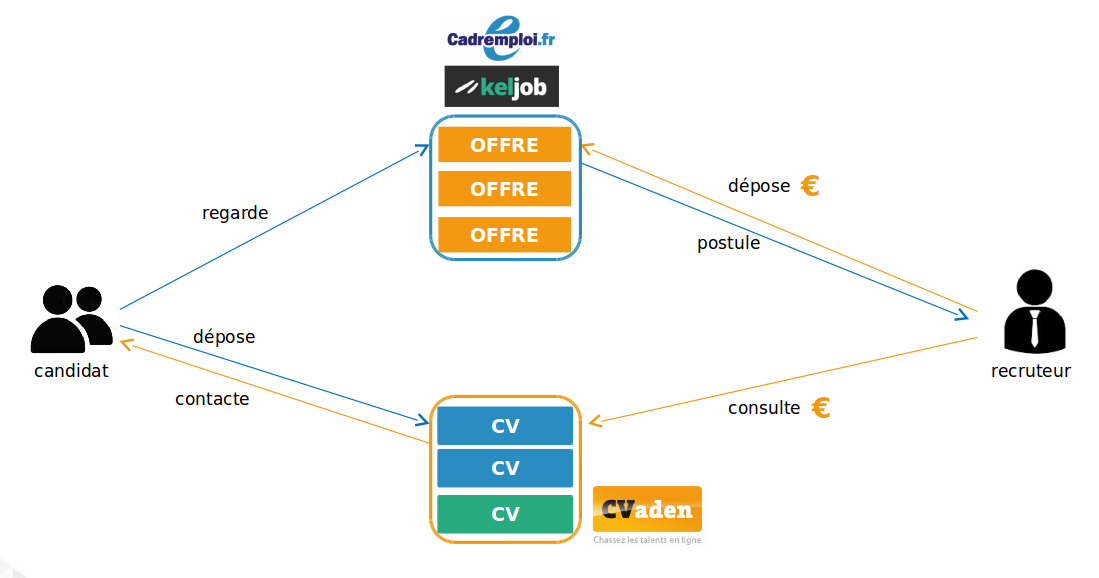
\includegraphics[width=1.25\textwidth]{Pictures/EmploiFCMS.png}
    \caption{Stratégie du secteur Emploi}
  \end{center}
\end{figure}
\begin{itemize}
  \item N°1 de l'Emploi privé sur Internet, avec les marques CADREMPLOI, KELJOB et CADRESONLINE
  \item N°1 de l'Emploi privé dans la presse nationale, avec LE FIGARO ECONOMIE
  \item N°1 de l'Emploi privé sur le Mobile, avec le succès des applications de CADREMPLOI et de KELJOB
\end{itemize}
Elle s'entoure aussi d'acteurs puissants dans le domaine de l'emploi, comme par exemple THE NETWORK, réseau international de recrutement N°1 (présent dans 136 pays).
Enfin, FIGARO CLASSIFIEDS se présente aussi comme un fournisseur de solutions RH, avec des produits comme CVAden (4 millions de CV), Adensourcing, CVmail ou Adenweb.
%--------------------------------------------------------------
\subsubsection{Formation}
Fort de son leadership et de son expertise sur le marché de l'Emploi, FIGARO CLASSIFIEDS a été l'un des pionniers sur le marché des annonces de formation sur Internet depuis 2004.
FIGARO CLASSIFIEDS peut ainsi accompagner les individus tout au long de leur carrière : formation initiale, en alternance, stages, recherche d'emploi, formation continue ou mobilité professionnelle via ses produits:
\begin{itemize}
  \item Le site Internet et l'application mobile de KELFORMATION
  \item Les rubriques « Formation » des sites CADREMPLOI, KELJOB et CADRESONLINE
  \item La CV-thèque Alternance de KELFORMATION
  \item Les titres de presse LE FIGARO, LE FIGARO ECONOMIE et LE FIGARO ETUDIANT
  \item La plateforme de vidéos CAMPUS CHANNEL
\end{itemize}
%--------------------------------------------------------------
\subsubsection{Immobilier}
À travers l'ensemble de ses médias, FIGARO CLASSIFIEDS dispose aussi d’une offre complète sur l’immobilier:
\begin{itemize}
  \item L’Ancien, avec EXPLORIMMO, PROPRIETES DE FRANCE, et LE FIGARO
  \item Le Neuf, avec EXPLORIMMONEUF
  \item Les Loisirs, avec BELLES MAISONS A LOUER
  \item Les Solutions, avec IMMOVISION (logiciel de transactions, référencement, digital agency…)
\end{itemize}

%--------------------------------------------------------------
\subsection{Métiers}
On retrouve différents corps de métiers dans cette entreprise, puisque 5 grandes directions se côtoient:  Digital, Marketing, Communication et Édition, Ressources Humaines et Contrôle de Gestion.
Toutes sont présentes au même étage des locaux du FIGARO, ce qui permet une intéraction simplifiée.
Je faisais partie, en ce qui me concerne, du pôle Digital dirigé par Laurent CHOLLAT-NAMY.

%--------------------------------------------------------------
\section{L'environnement de travail}
%--------------------------------------------------------------
\paragraph{}
Situés au cœur de Paris, dans le quartier de l’Opéra, les locaux du siège social de FIGARO CLASSIFIEDS reflètent une volonté commune : des locaux fonctionnels, créateurs d’échanges et de rencontres pour favoriser le travail collaboratif sous la forme d'open space à taille humaine.
Puisque FIGARO CLASSIFIEDS est la fusion de plusieurs startups, un effort de maintient de la proximité pareil à celui caractérisant les cultures d'entreprise originelles a été fait.
Toutes les strates de la hiérarchie se croisent quotidiennement et partagent des moments conviviaux notamment lors de divers évènements.
%--------------------------------------------------------------
\paragraph{}
Que ce soit à Paris, Lille, Lyon, Strasbourg, Toulouse, Bordeaux, Nantes, Rennes, Aix-en-Provence ou Sophia-Antipolis, FIGARO CLASSIFIEDS se vante de pouvoir compter 88\% de collaborateurs satisfaits de leur environnement de travail et 85\% plébiscitant une bonne ambiance au sein de leur service.

%-------------------------------------------------------------------------------
\section{L'entreprise et son informatique}
%-------------------------------------------------------------------------------
L'informatique occupe une place très importante dans le département Digital de FIGARO CLASSIFIEDS.
Cette branche a majoritairement vocation a développer des applications web, c'est pourquoi de nombreux outils sont disponibles.

%-------------------------------------------------------------------------------
\subsection{Outils, technologies et méthodes}
\label{subs:Outils, technologies et methodes}
%--------------------------------------------------------------
\paragraph{}
La plupart des employés a accès à un ordinateur, et un compte est attribué à l'arrivé, permettant de gérer notamment les emails ou la pose de jours de congés.
Les développeurs sont pour la majorité sous Ubuntu et développent via l'IDE IntelliJ Idea pour lequel une license est disponible.
L'utilisation de l'ordinateur à disposition est plutôt libre, puisqu'il est permis d'installer des logiciels sans avoir à passer par des Demandes de Prestation Informatique.
%--------------------------------------------------------------
\paragraph{}
La majorité des équipes échelonne sa mise en production sous plusieurs étapes en déployant une nouveauté sur des serveurs internes particuliers avant de procéder au déploiement public.
Cela permet de sécuriser les nouvelles versions du logiciel puisqu'il est ainsi possible de s'apercevoir d'un problème avant qu'il ne soit visible par le public.

%--------------------------------------------------------------
\subsection{Outils de travail collaboratifs}
\label{subs:Outils de travail collaboratifs}
Des outils sont aussi disponibles pour permettre aux équipes de travailler ensemble plus facilement.
%--------------------------------------------------------------
\paragraph{Redmine}
\label{par:Redmine}
\begin{wrapfigure}{l}{0.3\textwidth}
  \begin{center}
    
\includegraphics[width=0.20\textwidth]{Pictures/redmine_logo.png}
  \end{center}
\end{wrapfigure}
Redmine est un logiciel de gestion de projet open source utilisé chez Figaro CLASSIFIEDS pour notamment lister les demandes client et qui permet de rendre compte en ligne du travail effectué.
Lorsque l'on s'occupe d'une tâche, qu'on la termine ou que l'on a besoin de plus de renseignement, on le mentionne sur Redmine, ce qui permet de centraliser l'information et de la rendre disponible au reste de l'équipe.
%-------------------------------------------------------------------------------
\paragraph{Git}
\label{par:Git}
\begin{wrapfigure}{r}{0.3\textwidth}
  \begin{center}
    
\includegraphics[width=0.30\textwidth]{Pictures/git_logo.jpg}
  \end{center}
\end{wrapfigure}
Git est un outil de gestion de versions.
Il est aussi utilisé au sein du pôle Média pour mettre en commun le code écrit par toute l'équipe.
Il s'agit d'un outil que j'avais déjà beaucoup utilisé à l'EISTI mais d'une façon très simpliste, et j'ai appris au cours de mon stage de nombreuses nouvelles possibilités d'utilisation pour cet outil que nous n'avions jamais exploité à l'école.
%-------------------------------------------------------------------------------
\paragraph{Slack}
\label{par:Slack}
\begin{wrapfigure}{l}{0.3\textwidth}
  \begin{center}
    
\includegraphics[width=0.20\textwidth]{Pictures/slack_logo.png}
  \end{center}
\end{wrapfigure}
Au cours de mon stage, l'équipe Cadremploi au sein de laquelle je travaille s'est aussi mise à utiliser Slack, une sorte d'application de messagerie assez informelle qui permet de centraliser les échanges de l'équipe en un seul endroit.
Slack dispose d'un outil de recherche par mot clef très performant qui le rend donc très utile pour rechercher une information.
L'application permet aussi l'intégration de nombreux services dont Git, Jenkins ou Hangout, ce qui permet aussi une centralisation d'informations connexes utiles au projet en général.
Il s'agit d'un outil que j'ai utilisé avec mon équipe au cours de mon PFE et qui s'est avéré très simple d'utilisation et très utile pour partager de l'information.


%-------------------------------------------------------------------------------
\section{L'environnement de travail}
%-------------------------------------------------------------------------------
Le pôle média de FIGARO CLASSIFIEDS se présente comme un énorme open space dans lequel plusieurs équipes évoluent.
Bien que le nombre de service dans le bâtiment soit important, les relations n'y ont jamais été tendues.
Les membres des nombreuses équipes, se côtoient sereinement, se respectent et s'entraident.
J'ai réelement apprécié cette ambiance, et tout au long de mon stage je suis venu travailler dans un bon état d'esprit, sans contrainte mais avec au contraire beaucoup de plaisir.

%--------------------------------------------------------------
\subsection{Mon intégration}
\label{sub:Mon intégration}
Mon intégration au sein de l'équipe Cadremploi s'est très bien déroulée et l'accueil a été réussi.
L'organisation de séances sportives (escalade, Insanity, ...) ou d'afterworks a d'ailleurs aidé à souder cette équipe jeune et m'a aussi permis de rencontrer des gens dans des circonstances qui facilitent la mise en place de bonnes relations.
D'autre part, il est courant de voir les membres de la direction et bien qu'un respect s'impose, le contact est plutôt détendu.

%--------------------------------------------------------------
\subsection{Mon équipe: Cadremploi}
\label{sub:Mon équipe}
%--------------------------------------------------------------
\paragraph{}
J'ai effectué mon stage au sein de la très sympathique équipe Cadremploi qui est constituée de 9 personnes. Laëtitia Bukiatme est la Project Owner de l'équipe, Arnaud Brégère et Mathias Balussou sont deux développeurs front-end, Mickaël Barroux, Ludovic Iggiotti, Vincent Damery et Brice Friedrich sont développeurs Backend, tout comme Gaël Lazzari, techlead de l'équipe et Laurent Pageon mon maître de stage.
Cette équipe avait pour tâche à mon arrivée de sortir une nouvelle version pour l'espace recruteur du site Cadremploi.
Il s'agit d'une plateforme permettant aux recruteurs de déposer leurs annonces pour que celles-ci soient visibles sur l'espace public du site cadremploi.fr.
A ce projet s'est ajouté la refonte de la Home de l'espace public du site cadremploi.fr fin août auquel j'ai aussi participé.
%--------------------------------------------------------------
\paragraph{}
Mon équipe, très ouverte, est resté disponible tout au long de mon stage pour répondre à mes questions et m'aider lorsque j'en avais besoin.
On ressent que l'entraide y est un élément important.

% Chapter 3

\chapter{Être développeur à Cadremploi} % Main chapter title

\label{apports} % For referencing the chapter elsewhere, use \ref{apports_techniques}

\lhead{Troisième partie. \emph{Être développeur à Cadremploi}} % This is for the header on each page - perhaps a shortened title

%----------------------------------------------------------------------------------------
%----------------------------------------------------------------------------------------
\paragraph{}
Le site Cadremploi.fr est découpé en différentes parties qui sont en réalité des applications à part.
La partie publique est celle dans laquelle un utilisateur peut rechercher une offre en fonction de critères et y postuler.
Une seconde partie, destinée aux recruteurs, leur permet de saisir une offre d'emploi qui sera ensuite consultable depuis la partie publique.
J'ai travaillé durant ce stage sur la partie concernant les recruteurs, ou "Espace Recruteur".
Il était en effet à mon arrivée difficilement maintenable, utilisable et son interface était obsolète.
Une refonte totale en était nécessaire.
\paragraph{}
Mon stage consistait ainsi à participer avec l'équipe Cadremploi à la création d'un nouvel Espace Recruteur, plus moderne.
Je vais détailler dans cette partie le fonctionnement du nouvel espace recruteur ainsi que la façon dont l'équipe s'est organisé pour le développer.


\section{Cahier des charges et fonctionnement général du cycle de développement}
%----------------------------------------------------------------------------------------
\subsection{Contenu du stage}
\label{sub:Contenu du stage}

Le sujet principal de mon stage concernait la refonte de l'espace recruteur du site cadremploi.fr.
CADREMPLOI.fr a conçu un espace réservé aux professionnels afin de les aider dans leurs campagnes de recrutement.
Grâce à ce service de e-commerce, il leur est possible d'accéder à tous les produits et services qu'offre Cadremploi et de payer directement en ligne avec leur carte de crédit ou par chèque après réception de la facture.
%%%%%%%%%%%TODO%%%%%%%%%%%%%%%%%%%%%%
Cette application web avait déjà fait l'objet d'un développement il y a BLABLA ans et une refonte totale en était nécessaire, de manière à proposer des services nouveaux ainsi qu'un design plus actuel.
Concrètement, les principaux objectifs de ce stage étaient les suivants:
\begin{itemize}
  \item{} Développer de nouvelles fonctionnalités dans un environnement technique dynamique (Play! Scala, ElasticSearch, AngularJS)
  \item{} Maintenir le haut niveau de qualité et de tests présents
  \item{} Participer aux ateliers d'architecture et de cadrages techniques
  \item{} Echanger autour de bonnes pratiques avec les équipes de développement
\end{itemize}
%%%%%%%%%%%TODO%%%%%%%%%%%%%%%%%%%%%%
Les fonctionnalités attendues comprenaient notamment la mise en place du pattern Event Sourcing, que je détaillerai plus tard, de manière à pouvoir suivre de manière rigoureuse l'évolution de chaque utilisateur dans l'espace recruteur, ainsi que la simplification du système de classification des offres en créant un produit \"de base\" auquel se grefferont des options.

%----------------------------------------------------------------------------------------
\subsection{Méthodologie de management}
\label{sub:Méthodologie de management}
\paragraph{}
L'équipe Cadremploi, sur le projet Espace Recruteur notamment, suit une méthodologie Agile.
%%%%%%%%%%%TODO%%%%%%%%%%%%%%%%%%%%%%
% Bref résumé de ce qu'est la méthode Agile

% Rappel, MEP chaque semaine + MEPs exceptionnelles, sprint de 2 semaines
Le système de tickets post-it, des stand-up-meeting était très bien suivi bien que leur pratique ne soit pas un exercice figé.
Le contenu des stand-up-meeting est par exemple passé au cours de mon stage de "Qu'est-ce que j'ai fait?, Qu'est-ce que je vais faire?" à des questions plus pratiques: "Qu'est-ce que j'ai fait de réellement impactant pour le reste de l'équipe? Quels dysfonctionnements ai-je remarqué?".
Finalement, plutôt que l'évolution de chacun dans sa tâche, c'est l'évolution de l'application elle-même qui était alors discutée durant les stands-up, réduisant ainsi le temps de l'exercice, ce qui était nécessaire dans cette équipe de 10 personnes.
\paragraph{}
Les post-its suivaient un cycle de vie dont les étapes rentraient dans les catégories suivantes:
\begin{itemize}
  \item{Nouveau}, il s'agit du statut des tickets qui viennent d'arriver sur le tableau et qui seront donc à traiter prochainement
  \item{En cours}, il s'agit d'un ticket qu'un membre de l'équipe est en train de traiter.
  \item{Recette équipe}, lorsqu'une tâche est terminée, elle doit être validée par un membre de l'équipe; ce système de team review que je traiterai plus tard permet d'éviter de nombreuses erreurs au cours du développement de l'application.
  \item{Recette PO} lorsque le ticket passe l'étape de recette équipe, il arrive en recette PO.
  Le Project Owner s'occupe donc de vérifier que les modifications apportées correspondent bien aux attentes et qu'elles ne perturbent pas les anciennes fonctionnalités.
  Si un problème est rencontré, le PO rédige ses retours et la personne responsable du ticket se charge de corriger les problèmes.
  Le ticket reste dans le même état mais un jeu d'étiquettes "Retours Recette" et "Corrigé" est déposé sur le ticket pour qu'il soit possible de suivre l'évolution des corrections.
  \item{Validé}, le PO valide le ticket et les modifications seront mises en production sous peu
  \item{En attente}, le ticket ne peut être traité pour le moment; une synchronisation avec une autre équipe est nécessaire ou bien des questions restent sans réponse.
\end{itemize}
Ainsi les membres de l'équipe choisissent arbitrairement un ticket qu'il traitent en collant une étiquette les représentant dessus et déplacent le ticket dans la catégorie à laquelle il correspond.
\paragraph{}
Le tableau sur lequel sont affiché les tickets sont plutôt grands et plusieurs méthodes sont utilisés pour permettre à l'équipe de s'y retrouver rapidement.
En effet, en plus des colonnes de catégories dans lesquelles sont rangés les tickets, un code couleur permettait de différencier les tâches techniques des tâches fonctionnelles, ainsi que les tâches traitant de parties de Cadremploi autre que l'espace recruteur (projet de refonte de la Home, ...).
De plus, de petites étiquettes, en plus de celles représentant les membres de l'équipe, sont placées sur les tickets et permettent d'indiquer facilement si un des posts-its représente une tâche qui doit être mise en production dans la semaine (Cible MEP), ou si des retours suite à une recette (équipe ou PO) sont à traiter.
\paragraph{}
Enfin, les post-its représentant nos tâches rédigés sur un tableau se trouvent aussi référencés sur l'outil Redmine, une application web de gestion de projets, qui stocke toutes les informations concernant une tâche donnée.
Ce stockage double de l'information est un peu lourd; en effet, il est nécessaire de déplacer le ticket sur le tableau et d'effectuer le même changement en ligne sur Redmine.
Le point positif est qu'il permet à toute l'équipe, même en télétravail, d'accéder facilement à l'information concernant une tâche, notamment aux différentes discussions ayant eu lieu concernant cette tâche.
Il est cependant nécessaire de conserver l'affichage au tableau puisqu'il est bien plus visuel et permet à l'équipe d'échanger bien plus facilement que si le support était uniquement digital.

\section{Cahier des charges et fonctionnement général du cycle de développement}
%-------------------------------------------------------------------------------
\subsection{Contenu du stage}
\label{sub:Contenu du stage}
Le sujet principal de mon stage concernait ainsi la refonte de l'Espace Recruteur du site cadremploi.fr.
L'application actuelle se présente comme un espace réservé aux professionnels afin de les aider dans leur campagnes de recrutement.
Grâce à ce service de e-commerce, il leur est possible d'accéder à tous les produits et services qu'offre Cadremploi et de payer directement en ligne avec leur carte de crédit ou par chèque après réception de la facture.
Cette application web avait déjà fait l'objet d'un développement il y a plusieurs années et une refonte totale en était nécessaire, de manière à proposer des services nouveaux, un design plus actuel et des éléments de maintenabilité plus importants.
Concrètement, les principaux objectifs de ce stage étaient les suivants:
\begin{itemize}
  \item{} Développer de nouvelles fonctionnalités dans un environnement technique dynamique (Play! Scala, ElasticSearch, AngularJS)
  \item{} Maintenir le haut niveau de qualité et de tests présents
  \item{} Participer aux ateliers d'architecture et de cadrages techniques
  \item{} Echanger autour de bonnes pratiques avec les équipes de développement
\end{itemize}
\begin{figure}[h]
  \begin{center}
    \hspace*{-1in}
    
\includegraphics[width=1\textwidth]{Pictures/EspaceRecruteur.png}
  \end{center}
\end{figure}

%-------------------------------------------------------------------------------
\subsection{Méthode de management}
\label{sub:Méthode de management}
%-------------------------------------------------------------------------------
\paragraph{}
L'équipe Cadremploi, sur le projet Espace Recruteur notamment, suit une méthodologie Agile.
Les méthodes de type agile se veulent plus pragmatiques que les méthodes traditionnelles.
Elles impliquent au maximum le client et permettent une grande réactivité à ses demandes.
Les méthodes agiles prônent 4 valeurs fondamentales: l'équipe, qui doit être soudée et dans laquelle la communication est fondamentale, le fonctionnement de l'application, la collaboration avec les clients au delà de la négociation contractuelle ainsi que la flexibilité de la structure du logiciel, acceptant ainsi aisément le changement.
Pour l'équipe Cadremploi, cela se caractérisait par des meetings quotidien devant un tableau rassemblant des tâches demandées par le client écrites sur des post-its, une mise en production des nouveautés développées chaque jeudi, la mise en place de tests unitaires et end-to-end ainsi que des revues de code pour chaque tâche effectuée.
%-------------------------------------------------------------------------------
\paragraph{Le stand-up meeting}
Comme dans de nombreuses méthodes Agiles, la communication au sein de l'équipe passe notamment par un stand-up-meeting quotidien ainsi qu'un affichage mural composé de posts-its représentant les tâches relatives à l'évolution de l'application.
Le système de tickets post-it, des stand-up-meeting était très bien suivi bien que leur pratique ne soit pas un exercice figé.
Le contenu des stand-up-meeting est par exemple passé au cours de mon stage de "Qu'est-ce que j'ai fait?, Qu'est-ce que je vais faire?, Ai-je des problèmes?" à des questions plus pratiques: "Qu'est-ce que j'ai fait de réellement impactant pour le reste de l'équipe? Quels dysfonctionnements ai-je remarqué?".
Finalement, plutôt que l'évolution de chacun dans sa tâche, c'est l'évolution de l'application elle-même qui était alors discutée durant les stands-up, réduisant ainsi le œtemps de l'exercice, ce qui était une nécessité dans cette équipe de 10 personnes.
De plus, suite à un amoncellement de tâches trop important qui produisait un confus global lors de la lecture du tableau, il a été mis en place des règles permettant de limiter le nombre de tickets en cours de traitement, permettant une meilleure organisation de l'équipe.
%-------------------------------------------------------------------------------
\paragraph{Cycle de vie d'une tâche}
Les post-its suivaient un cycle de vie dont les étapes rentraient dans les catégories suivantes:
\begin{itemize}
  \item "Nouveau", il s'agit du statut des tickets qui viennent d'arriver sur le tableau et qui seront donc à traiter prochainement
  \item "En cours", il s'agit d'un ticket qu'un membre de l'équipe est en train de traiter.
  \item "Recette" équipe, lorsqu'une tâche est terminée, elle doit être validée par un membre de l'équipe.
  Ce système de team review permet d'éviter de nombreuses erreurs au cours du développement de l'application: une vérification du code ainsi que des tests écrits sont effectués.
  \item "Recette" PO lorsque le ticket passe l'étape de recette équipe, il arrive en recette PO.
  Le Project Owner s'occupe donc de vérifier que les modifications apportées correspondent bien aux attentes et qu'elles ne perturbent pas les anciennes fonctionnalités.
  Si un problème est rencontré, le PO rédige ses retours et la personne responsable du ticket se charge de corriger les problèmes.
  Le ticket reste dans le même état mais un jeu d'étiquettes "Retours Recette" et "Corrigé" est déposé sur le ticket pour qu'il soit possible de suivre l'évolution des corrections.
  \item "Validé", le PO valide le ticket et les modifications seront mises en production sous peu
  \item "En attente", le ticket ne peut être traité pour le moment; une synchronisation avec une autre équipe est nécessaire ou bien des questions restent sans réponse.
\end{itemize}
Ainsi les membres de l'équipe choisissent arbitrairement un ticket qu'il traitent en collant une étiquette, un autocollant les représentant dessus et déplacent le ticket dans la catégorie à laquelle il correspond.
Les tickets validés sont généralement mis en production chaque semaine, le jeudi, à l'exception de quelques mises en productions (MEP) exceptionnelles.
\paragraph{Organisation du tableau}
Le tableau sur lequel sont affichés les tickets est plutôt grand et plusieurs méthodes sont utilisées pour permettre à l'équipe de s'y retrouver rapidement.
En effet, en plus des colonnes de catégories dans lesquelles sont rangés les tickets, un code couleur permettait de différencier les tâches techniques des tâches fonctionnelles, ainsi que les tâches traitant de parties de Cadremploi autre que l'espace recruteur (projet de refonte de la Home, ...).
De plus, de petites étiquettes, en plus de celles représentant les membres de l'équipe, sont placées sur les tickets et permettent d'indiquer facilement si un des posts-its représente une tâche qui doit être mise en production dans la semaine (Cible MEP), ou si des retours suite à une recette (équipe ou PO) sont à traiter.
\paragraph{Référencement des tâches}
Enfin, les post-its représentant nos tâches rédigées sur un tableau se trouvent aussi référencées sur l'outil Redmine, une application web de gestion de projets, qui stocke toutes les informations concernant une tâche donnée.
Ce stockage double de l'information est un peu lourd; en effet, il est nécessaire de déplacer le ticket sur le tableau et d'effectuer le même changement en ligne sur Redmine.
Le point positif est qu'il permet à toute l'équipe, même en télétravail, d'accéder facilement à l'information concernant une tâche, notamment aux différentes discussions ayant eues lieu concernant cette tâche.
Il est cependant nécessaire de conserver l'affichage au tableau puisqu'il est bien plus visuel et permet à l'équipe d'échanger bien plus facilement que si le support était uniquement digital.

\section{Aperçu des technologies et des techniques utilisées}

\subsection{Langages}
\label{sub:Langages}
\subsubsection{Backend}
\label{subs:Backend}
\begin{figure}[h]
  \begin{center}
    
\includegraphics[width=0.3\textwidth]{Pictures/play_logo.png}
    \hspace{1in}
    
\includegraphics[width=0.15\textwidth]{Pictures/scala_logo.png}
  \end{center}
\end{figure}

Le nouvel espace recruteur est géré en backend via le framework Play! dans sa dernière version (2.4.2) et sous le langage Scala.
Il s'agit d'un couple qui permet d'écrire du code rapidement et de façon maintenable.
Play est l'un des framework les plus connus dans le monde Java et offre de nombreux avantages:
\begin{itemize}
  \item Il supporte le rechargement à chaud.
  Il suffit de lancer Play via sa console en mode développement et il prendra automatiquement en compte à chaud les changements effectués sur le code, mais aussi les templates ou le routage.
  Cela contribue grandement au gain de productivité qu'offre Play.
  \item En plus de s’appuyer sur du code à typage statique, Play propose la sécurité du typage à d’autres endroits et notamment sur les templates ou sur le routage des différents contrôleurs.
  Un certain nombre de problèmes sont alors mis en lumière directement à l’étape de la compilation.
  \item Il permet d'exécuter des tests, notamment sur la couche web à plusieurs niveaux:
  On peut par exemple tester un contrôleur en démarrant un serveur web (donc via HTTP) ou, sans le démarrer, en appelant simplement le contrôleur avec le contexte qui va bien, le tout de manière simple et rapide à l’exécution.
  \item Il est sans état et basé sur des entrées sorties non bloquantes et permet ainsi une capacité à monter en charge très intéressante
  \item Il supporte nativement REST, JSON, Websocket entre autres et se présente donc comme un framework moderne
\end{itemize}
Un des points négatifs de ce choix en backend est l'utilisation de fait obligatoire de SBT qui nous a posé de nombreux problèmes.
En effet, cet outil était souvent lent, compliqué d'utilisation et ralentissait souvent le développement notamment via ses résolutions de dépendances interminables.
\subsubsection{Frontend}
\label{subs:Frontend}
\begin{figure}[h]
  \begin{center}
    
\includegraphics[width=0.4\textwidth]{Pictures/angular_logo.png}
  \end{center}
\end{figure}
%% TODO
Du côté front, l'équipe a utilisé le framework AngularJS ainsi que la librairie D3.js qui permettent des animations dynamiques.
Ce choix de technologie peut être soutenu pour les points suivants:
\begin{itemize}
  \item Angular permet une maintenabilité de l'application aisée, notamment en demandant une structure de type MVC au développeur, ainsi qu'en utilisant du HTMl, qui est déclaratif, pour définir l'interface utilisateur.
  \item Il s'agit de plus d'un framework flexible puisqu'il est possible de composer une application en
\end{itemize}

\subsection{Environnements et outils}
\paragraph{IntelliJ}
\label{par:IntelliJ}
\begin{wrapfigure}{l}{0.15\textwidth}
  \vspace{-2.5em}
  \begin{center}
    
\includegraphics[width=0.15\textwidth]{Pictures/intellij_logo.png}
  \end{center}
\end{wrapfigure}
Le développement de l'espace recruteur s'est fait sous le framework Play! et IntelliJ Idea était l'IDE utilisé par l'équipe pour développer, puisqu'il offre une bonne intégration de ce framework.
J'avais déjà souvent utilisé cet IDE pour différents projets que j'ai eu à rendre tout au long de ma scolarité à l'EISTI, ainsi son utilisation ne m'a posé aucun problème.
\paragraph{Git}
\label{par:Git}
L'équipe étant nombreuse et l'application étant sujete à grossir avec le temps, un outil de gestion de versions a été utilisée.
Git est l'outil le plus répandu et le plus efficace connu, c'est ce que l'équipe Cadremploi a utilisé.
Il s'agissait aussi d'un outil que j'avais beaucoup utilisé mais de manière très simpliste et j'ai appris à m'en servir d'une toute autre façon, bien plus complète, pendant ce stage.
\paragraph{Jenkins}
\label{par:Jenkins}
\begin{wrapfigure}{rH}{0.25\textwidth}
  \begin{center}
    
\includegraphics[width=0.15\textwidth]{Pictures/jenkins_logo.png}
  \end{center}
\end{wrapfigure}
L'équipe Cadremploi utilise aussi Jenkins comme outil d'intégration continue pour déployer les nouveautés sur les différents environnement de production utilisés (recette, intégration), les mises en production et préproductions n'étant pas gérées directement par l'équipe.
Cet outil avait été brièvement présenté lors du cours d'Outils de Développement mais jamais utilisé.
Jenkins est un outil open source permettant de compiler et de tester un projet de manière continue.
Il aide de fait les développeurs à intégrer facilement des changements à une application.
Bien que nous avions été tenté de mettre en place un Jenkins avec mon équipe de Projet de Fin d'Étude, cela ne s'est jamais fait par manque de temps et puisqu'un besoin concret ne s'est jamais montré.
Je n'ai pas eu de mal à l'utiliser puisqu'une fois configuré, cet outil est réelement simple d'utilisation.
Plusieurs environnements de développement sont utilisés par Cadremploi comme pour les autres équipes de Figaro Classifieds:
\begin{itemize}
  \item{Environnement de développement}, où les développeurs postent régulièrement les améliorations qu'ils mettent en place. Jenkins n'est pas utilisé pour cet environnement puisque les changements y sont publiés directement via Git.
  \item{Environnement de recette}, où la Project Owner vérifie que les changements apportés fonctionnent effectivement et les valide.
  \item{Environnement de pré-production} qui est un environnement qui ressemble autant que possible à l'environnement de production et où sont surtout testés les architectures
  \item{Environnement de production} qui est la dernière étape, contenant l'application utlisée réelement par les utilisateurs
  \item{Environnement de'intégration}, il s'agit d'un environnement supplémentaire qui est préféré pour les tests fait sur l'infrastructure du projet.
\end{itemize}
J'ai été habitué durant ma scolarité à l'EISTI à utiliser la majorité des outils présentés précédemment puisque j'étais uniquement étranger à Jenkins.
J'ai malgré tout grandement progressé dans mon utilisation de ces outils et particulièrement pour Git que j'ai redécouvert; le projet auquel je participais differais grandement en taille de ceux auquels j'avais contribué auparavant.
%Potentiellement, Rundeck, Kibana, Puppet.

\section{Une équipe nombreuse}
\label{sec:Une équipe nombreuse}
Cadremploi, a mon arrivée, comptait alors 10 membres dont 9 développeurs.
Il s'agit d'une équipe d'une taille importante pour un projet Agile.
Ainsi, de l'organisation ainsi qu'une bonne coordination étaient nécessaires.

\subsection{Revue de code}
\label{sub:Revue de code}
Le développement d'applications demande très souvent à une équipe de personnes de travailler ensemble.
Plus l'équipe grandit plus il est compliqué de garantir une coordination correcte et une bonne organisation.
Les équipes d'ingénieur sont spécialement soumises à ce genre de problèmes puisque du code est quotidiennement partagé entre plusieurs personnes au sein d'une entreprise.
La revue de code aide à partager le savoir et les bonnes pratiques.
\paragraph{}
Le flux de production de l'équipe Cadremploi demande à chaque membre de l'équipe à passer un ticket terminé dans un état "R7 Equipe".
Le ticket doit alors être revu par un autre développeur de l'équipe.
Ce dernier doit analyser les changements fait au code, s'assurer qu'ils n'introduisent pas de troubles dans l'application et vérifier que le code produit suit bien les normes de code imposées par l'équipe.
\paragraph{}
La revue de code par d'autres membres de l'équipe offre de nombreux avantages autres qu'une simple vérification du code.
En effet, il est clair que n'avoir qu'un unique membre de l'équipe responsable d'un point critique sur l'application est dangereux.
La revue de code distribue le savoir au sein de l'équipe et permet d'informer plusieurs membres d'un changement.
De plus, elle stimule les conversations portant sur la structure du code, l'architecture de l'application et permet ainsi à de nouveaux venus, comme je l'étais, de s'adapter rapidement et donc de devenir productif plus rapidement.
\paragraph{}
Il ne m'est pas possible de réelement comparer ce mode de fonctionnement avec mes projets précédents.
En effet, mes projets passés se faisaient dans des équipes plus réduites, et le temps manquait pour la revue de code.
Cela ne nous empêchait pas de suivre la règle du boyscoot, qui prescrit de toujours laisser une fonction, un module dans un meilleur état que celui dans lequel on l'a trouvé, et qui évite la "possession" du code par un membre de l'équipe.
Cette règle est plus ou moins comprise dans la revue de code de Cadremploi qui offre plus d'avantages encore.

\subsection{Utilisation de Git}
\label{sub:utilisation de Git}
Git est un outil de contrôle de version flexible et puissant.
Il propose énormément d'options de workflow et il est parfois compliqué
Git is a flexible and powerful version control system. While Git offers significant functionality over legacy centralized tools like CVS and Subversion, it also presents so many options for workflow that it can be difficult to determine what is the best method to commit code to a project. The following are the guidelines I like to use for most software projects contained within a Git repository. They aren't applicable to every Git project (especially those hosted on drupal.org or GitHub), but I've found that they help ensure that our own projects end up with a reasonable repository history.

\section{Architecture de l'application}
\label{sec:Architecture de l'application}
%-------------------------------------------------------------------------------
L'espace recruteur dispose d'une architecture interne assez singulière et je n'avais jamais eu à faire à ce type d'application auparavant.
En effet, l'équipe Cadremploi a mis en place un modèle d'architecture de type CQRS couplé à une gestion d'état basé sur de l'Event Sourcing.
%-------------------------------------------------------------------------------
\paragraph{CQRS: Command Query Responsibility Seggregation}
\label{par:CQRS: Command Query Responsibility Seggregation}
Dans les systèmes de gestion de donnée traditionnels, les commandes, c'est à dire la mise à jour des données, et les requêtes son exécutées sur un seul regroupement d'entitées regroupées dans une unique base de donnée.
CQRS est un modèle d'architecture plutôt récent dont le principe repose, comme son nom l'indique, sur la séparation entre l'écriture et la lecture de l'information.
Nous avons suivi lors du développement de l'espace recruteur ce pattern puisque la séparation des composants de traitement (les "commands") et de restitution (les "queries") de l'information offrait une architecture très intéressante de laquelle nous avons tiré de nombreux bénéfices tels que la suppression du risque d'effets de bord ou l'allègement des classes de service.
%-------------------------------------------------------------------------------
\paragraph{Event Sourcing}
\label{par:Event Sourcing}
La gestion commune de l'état d'un système consiste à enregistrer l'état courant des objets le composant et de reporter chaque changement effectué sur le système en modifiant directement son état, notamment via une mise à jour en base de données.
L'idée fondamentale de l'Event Sourcing est d'assurer que chaque changement appliqué à l'état d'une application peut être capturée dans un objet de type événement.
Ce n'est plus l'état du système qui est enregistré mais les événements qui ont mené le système à l'état dans lequel il est actuellement.
Cette façon de penser permet notamment d'obtenir un log complet de tous les changements effectués, et donc une traçabilité ainsi qu'une aisance de debug importante.
Il est ainsi possible de pouvoir reconstruire tous les états passés de l'application.
%-------------------------------------------------------------------------------
\paragraph{}
Je vais présenter dans cette partie ce type singulier d'architecture qui permet de mettre en place un système extensible et distribuable.
J'expliquerai ensuite la façon dont elle a été mise en place sur la nouvelle version de l'espace recruteur de cadremploi.fr.

%-------------------------------------------------------------------------------
\input{"Chapters/Chapter3/architecture/organisation"}
\input{"Chapters/Chapter3/architecture/implementation"}
%-------------------------------------------------------------------------------

\section{Event sourcing}
% http://martinfowler.com/eaaDev/EventSourcing.html
% https://github.com/eventstore/eventstore/wiki/Event-Sourcing-Basics
Une des demandes pour le nouvel espace recruteur est de pouvoir suivre avec précision les actions de l'utilisateur.
Ainsi chaque modification qu'il apportera à une de ses offres ou à son profil par exemple doit être enregistrée.
%----------------------------------------------------------------------------------------
\textit{"L'idée fondamentale derrière l'Event Sourcing est d'assurer que chaque modification de l'état d'une application est capturée dans un objet événement et que ces événements sont eux-mêmes stockés dans l'ordre dans lequel ils ont été appliqués à l'application."} (Martin Fowler)
%----------------------------------------------------------------------------------------
\subsection{Fonctionnement désiré}
\label{sub:Fonctionnement desire}
Il est nécessaire de pouvoir suivre l'évolution de l'annonce que créé un utilisateur.
Concrètement, à chaque fois que l'utilisateur modifie son annonce, on veut générer un événement qui informe notre système de cette modification.
Toutes ces données pourront ainsi être utilisées pour faire des statistiques ainsi que des contrôles.
Une des utilités de ce suivi est par exemple de pouvoir contrôler les éditions abusives d'annonces déjà en ligne.
Il est ainsi possible de suivre de très près la façon dont l'utilisateur procède, ou les champs qui posent problème.

%----------------------------------------------------------------------------------------
\subsection{Fonctionnement technique}
%----------------------------------------------------------------------------------------
\subsubsection{Enregistrement de l'événement}
\label{subs:Enregistrement de l'evenement}
Concrètement, derrière chaque champ formulaire que l'utilisateur remplit, un watcher d'Angular est présent.
Ainsi lorsque ce watcher indique que le champ a été modifié, on récupère la valeur qu'il contient et envoyons cette demande de modification vers le backend.
Cette "demande de modification" est traitée comme une commande et génère alors un ou plusieurs événements qui résument la modification effectuée et sont stockés dans une base de donnée, conformément au modèle de Write du pattern CQRS décrit ci-dessus.
Chacune des modifications faite par l'utilisateur est ainsi enregistrée, et il est possible de connaître l'état du système à tout instant t donné en interrogeant la base de données.
%----------------------------------------------------------------------------------------
\subsubsection{Utilisation de l'événement}
\label{subs:Utilisation de l'evenement}
Si l'enregistrement en base se passe bien, l'événement est ensuite publié sur un EventBus, un objet Akka qui permet entre autre d'envoyer un message à des groupes d'acteurs, pour être écouté par des objets de type Projection.
Ces projections écoutent seulement une partie des événements selon leurs responsabilité et modifient en conséquence un objet DTO qu'elles indexent.
Ce traitement est fait de manière asynchrone, via le système d'acteurs Akka.
Il permet donc d'optimiser le modèle CQRS vu précédemment: la commande est exécutée rapidement puisque l'événement est sauvegardé de suite et le reste du traitement est effectué de manière asynchrone.
Cela permet d'informer quasi instantannément l'utilisateur que son action a été prise en compte.
D'autre part, en acceptant de rendre asynchrone et donc pas forcément instantannée la mise à jour de la partie Read du modèle, on améliore grandement la performance ressentie par l'utilisateur.
Le système est donc tenu à jour en lecture et ainsi, à l'appel d'une query, les projections peuvent être interrogées pour récupérer la donnée de manière très rapide.


\section{Domain Driven Development}


%----------------------------------------------------------------------------------------
%----------------------------------------------------------------------------------------
\section{Organisation}
comparaison entre les plannings prévisionnels et réels

%----------------------------------------------------------------------------------------

%----------------------------------------------------------------------------------------
%----------------------------------------------------------------------------------------

\section{Auto-évaluation}
respect des délais, autonomie, qualité du travail, apports à l'équipe

%----------------------------------------------------------------------------------------
%----------------------------------------------------------------------------------------

\section{Résultats et prolongements possibles}
le site tourne et continuera de fonctionner encore

%----------------------------------------------------------------------------------------

% Chapter 4

\chapter{Le stage dans ma formation} % Main chapter title

\label{formation} % For referencing the chapter elsewhere, use \ref{Chapter1}

\lhead{Quatrième partie. \emph{Le stage dans ma formation}} % This is for the header on each page - perhaps a shortened title

%----------------------------------------------------------------------------------------

\section{Ce qui m'a été le plus utile dans ma formation}
J'ai pu voir lors de mon stage l'utilité des cours suivis à l'EISTI qui se sont montrés tant utiles qu'actuels.
En effet, je n'ai utilisé que très peu d'outils ou de technologies dont je n'avais jamais entendu parler
Scala, Akka, Veille technologique

%----------------------------------------------------------------------------------------

\section{Ce que m'a apporté ce stage pour le reste de ma carrière}
Git, veille technologique, architecture, scala

%% Chapter 5

\chapter{Le stage dans ma formation} % Main chapter title

\label{formation} % For referencing the chapter elsewhere, use \ref{Chapter1}

\lhead{Quatrième partie. \emph{Le stage dans ma formation}} % This is for the header on each page - perhaps a shortened title

Durant ma formation, j’ai acquis beaucoup de connaissances théoriques et ai pu mettre en pratique certaines d’entre elles lors de projets ou TP.
Répondre à la demande d’un client dans les délais impartis, communiquer ses idées et travailler en équipe avec des partenaires variés tels sont les objectifs du stage.


%---------------------------------------------------------------
%---------------------------------------------------------------
\section{Les apports de ma formation}

%---------------------------------------------------------------
\subsection{Programmation Scala et Framework Play}
\label{sub:Programmation Scala et Framework Play}
%---------------------------------------------------------------
\paragraph{}
La majorité du code que j'ai eu à écrire durant ce stage l'a été en Scala sous le framework Play, ainsi les deux cours en traitant m'ont été vraiment utiles.
Plus que de simplement me servir de ce que j'avais appris, ils ont été une base grâce à laquelle j'ai pu continuer à apprendre via des blogs ou des conférences en ligne.
Il m'a permis de progresser tant au niveau de la clarté de l'écriture du code qu'en connaissance sur les structures et les singularités que ce couple de technologies présente.
%---------------------------------------------------------------
\paragraph{}
De plus, il m'a sensibilisé à l'utilisation de structures fonctionnelles, plus lisibles, courtes et explicites que les structures habituelles que l'on peut rencontrer dans un langage orienté objet.
Ce point est primordial lorsque l'on travail au sein d'un projet avec d'autres personnes puisque ce qui est écrit est très succeptible d'être repris plus tard par d'autres personnes.

%---------------------------------------------------------------
\subsection{Angular}
\label{sub:Angular}
La partie Frontend de l'application Espace Recruteur demandait l'utilisation d'Angular et ce cours m'a permis, sans réels problèmes, de participer à son écriture, même si la majorité de mes apports au projet se faisaient en backend.
En effet, en plus de simplement cabler les parties client et serveur de l'application, et de me cantonner au traitement des tâches backend, j'ai su, en grande partie grâce à ce cours, apporter mon aide pour l'implémentation de la partie front.
J'ai en effet pu être rapidement à l'aise avec cette partie de l'application.

%---------------------------------------------------------------
\subsection{Enjeux et perspectives du Cloud Computing}
\label{sub:Enjeux et perspectives du Cloud Computing}
%---------------------------------------------------------------
\paragraph{}
Ce cours avait pour but d'inciter à la veille technologique via la présentation de contenus vidéos ou audios dont le sujet portait sur les nouvelles technologies.
Il m'a poussé à m'intéresser à différentes technologies, à faire des recherches sur les technologies que je ne maîtrisais pas encore (Kafka, ELasticSearch, ...), mais aussi sur celles que je commençais à maîtriser pour aller plus loin encore (Scala, Git, Akka, ...).
%---------------------------------------------------------------
\paragraph{}
C'est entre autre avec ce cours quelque peu spécial que j'ai commencé à prendre l'habitude de lire sur des nouveautés, des blogs d'experts du web et ainsi voir leur avis sur de nombreux outils qui étaient utilisés aussi chez FIGARO CLASSIFIEDS.
Il a été une aide à la construction d'un avis sur plusieurs technologies et méthodes utilisées dans l'équipe.
%---------------------------------------------------------------
\paragraph{}
Enfin, ils ont été une sorte d'introduction aux architectures où de nombreuses technologies se croisent, puisqu'on s'éloigne des structures avec trois composants: frontend, backend et base de données pour quelque chose de plus souple mais aussi de plus efficace puisque des technologies dédiées sont utilisées pour des points particuliers, ce qui permet de gagner grandement en performance.

%---------------------------------------------------------------
\subsection{Autres}
\label{sub:Autres}
%---------------------------------------------------------------
\paragraph{}
De manière plus générale mais néanmoins importante, les différents projets, notamment de fin de 2e année et ceux de de 3e année (le PFE et l'application en partenariat avec CDiscount), ont été de belles occasions de travailler en équipe, de mettre en place des méthodes et d'expérimenter.
Ces projets m'ont ainsi beaucoup apporté en confiance quant à mes compétences mais aussi m'ont permis de m'exercer de façon concrète sur des technologies en dehors des cours parfois trop théoriques.
%---------------------------------------------------------------
\paragraph{}
Les cours de sécurité que j'ai suivi durant mon semestre de mobilité à Heriott Watt ainsi que durant ma dernière année à l'EISTI m'ont appris à repérer des failles courantes et à les éviter durant mon développement, ainsi qu'à en informer les autres.

%---------------------------------------------------------------
%---------------------------------------------------------------
\section{Les apports de mon stage pour le monde du travail}
%---------------------------------------------------------------
\subsection{Méthodes de travail}
\label{sub:Méthodes de travail}
%---------------------------------------------------------------
\paragraph{}
Ce stage était pour moi un premier vrai pas dans le monde du web en entreprise.
Il était donc une occasion de consolider mes bases en utilisant des technologies nouvelles.
Il a évidement été un test en soi de mes compétences, du niveau que j'ai atteint et de ma capacité à répondre à des requêtes, dans une structure et des enjeux plus grands que ce que j'avais pu expérimenter avec mes groupes de projets à l'EISTI.
C'est ainsi avec des exigences de respect de planning, des contraintes financières, dans un environnement de travail qui n'était pas celui que j'avais moi-même mis en place et avec des gens que je ne connaissais initialement pas que j'ai dû évoluer.
Ce fut donc une mesure concrète de la qualité de mes méthodes de travail et de leur mise en place dans un environnement nouveau autant qu'une prise de conscience concrète des besoins technologiques nombreux que demande la construction d'une application Web destinée à un public nombreux.
%---------------------------------------------------------------
\paragraph{}
Durant ce stage de fin d'étude, j'ai réalisé des tâches comme tout membre de l'équipe l'aurait fait et la prise de responsabilité a été bien plus grande que lors de mon stage de deuxième année.
La mise en place d'une nouveauté pouvait impacter dès la semaine suivante l'application en production, mais aussi directement mon équipe et il m'a été donc nécessaire de m'appliquer réellement, de mettre en place des tests, des vérifications importantes avant d'assurer la complétion d'une tâche.
Cette rigueur que je n'avais pas encore complètement a été un des grands apports de ce stage, en dehors des compétences technologiques et architecturales que j'ai pu développer.

%---------------------------------------------------------------
\subsection{Les acteurs de la création d'un produit}
\label{sub:Les acteurs de la création d'un produit}
Les réunions auxquelles j'ai assisté pendant mon stage, qu'il s'agisse de réunions d'information sur le plan marketing ou un rassemblement d'équipe pour débattre sur la stratégie à adopter pour une nouveauté, ont été très instructives.
Elles ont été une démonstration très intéressante des acteurs intervenant au cours de la mise en place d'un projet, d'un point de vue global, mais aussi des différents points de vue qu'il est possible d'adopter sur l'architecture d'une application comme l'est l'Espace Recruteur.
Interagir avec tous ces acteurs, les observer et travailler à leur côté a été une expérience réellement enrichissante.

%---------------------------------------------------------------
\section{Conclusion}
Ce stage m'a permis d'appliquer la théorie des cours au monde professionnel ainsi que de découvrir de nouvelles technologies et développer mes compétences.
L'Option Ingénierie du Cloud Computing que j'ai suivie cette année a été un choix pertinent puisqu'il m'a mené dans une direction professionnelle qui correspond à mes objectifs: travailler dans un environnement novateur et dans lequel je puisse continuer d'apprendre et m'épanouir tant professionnellement que personnellement.

%\input{Chapters/Chapter6}
%\input{Chapters/Chapter7}

%----------------------------------------------------------------------------------------
%	THESIS CONTENT - APPENDICES
%----------------------------------------------------------------------------------------

\addtocontents{toc}{\vspace{2em}} % Add a gap in the Contents, for aesthetics

\appendix % Cue to tell LaTeX that the following 'chapters' are Appendices

% Include the appendices of the thesis as separate files from the Appendices folder
% Uncomment the lines as you write the Appendices

%% Appendix A

\chapter{Appendix Title Here} % Main appendix title

\label{AppendixA} % For referencing this appendix elsewhere, use \ref{AppendixA}

\lhead{Appendix A. \emph{Appendix Title Here}} % This is for the header on each page - perhaps a shortened title

Write your Appendix content here.
%\input{Appendices/AppendixB}
%\input{Appendices/AppendixC}

\addtocontents{toc}{\vspace{2em}} % Add a gap in the Contents, for aesthetics

\backmatter

%----------------------------------------------------------------------------------------
%	BIBLIOGRAPHY
%----------------------------------------------------------------------------------------

\label{Bibliography}

\lhead{\emph{Bibliography}} % Change the page header to say "Bibliography"

\bibliographystyle{unsrtnat} % Use the "unsrtnat" BibTeX style for formatting the Bibliography

\bibliography{Bibliography} % The references (bibliography) information are stored in the file named "Bibliography.bib"

\end{document}
